\section{Opgave 1 - MeeMoo state machine}
\begin{enumerate}
	\item[1)]
	
	Som anmodet i opgavebeskrivelsen, har vi skrevet programmet som en Moore state machine først. Altså, ændrer Moore output værdi, alt efter hvilken state den skiftes til. Denne værdi er clock-reguleret.
	
	Derefter har vi tilføjet Mealy state machinen inde i state-init, hvor den regulerer Mealy output værdien efter værdierne for A og B. Denne værdi er IKKE clock-reguleret.
	VHDL-koden for programmet er følgende:
	
\begin{lstlisting}[caption={Kode for MeeMoo state machine},label={lst:MeeMooSM}]
library ieee;
use ieee.std_logic_1164.all;

entity MeeMooSM is
port (clk, reset, a, b : in std_logic;
moo_out, mee_out : out std_logic);
end MeeMooSM;

architecture three_processes of MeeMooSM is
type state is (state_idle, state_init, state_active);
signal present_state, next_state : state;
begin

state_reg: process (clk, reset)
begin
if reset = '0' then
present_state <= state_idle;
elsif rising_edge(clk) then
present_state <= next_state;
end if;
end process;

outputs: process (present_state, a, b)
begin	
case present_state is
when state_idle => 
moo_out <= '0';
mee_out <= '0';
when state_init => 
moo_out <= '1';
if a = '0' and b = '1' then
mee_out <= '0';
elsif a = '1' and b = '1' then
mee_out <= '1';
end if;
when others => 
moo_out <= '1';
mee_out <= '0';
end case;
end process;

nxt_state: process (present_state, a, b)
begin
case present_state is
when state_idle =>
if b = '0' then
next_state <= state_idle;
elsif b = '1' then
next_state <= state_init;
end if;
when state_init =>
if a = '0' and b = '0' then
next_state <= state_idle;
elsif a = '1' and b = '0' then
next_state <= state_active;
else 
next_state <= state_init;
end if;
when state_active =>
next_state <= state_idle;
end case;
end process;
end three_processes;

\end{lstlisting}

\begin{figure}[h]
	\centering
	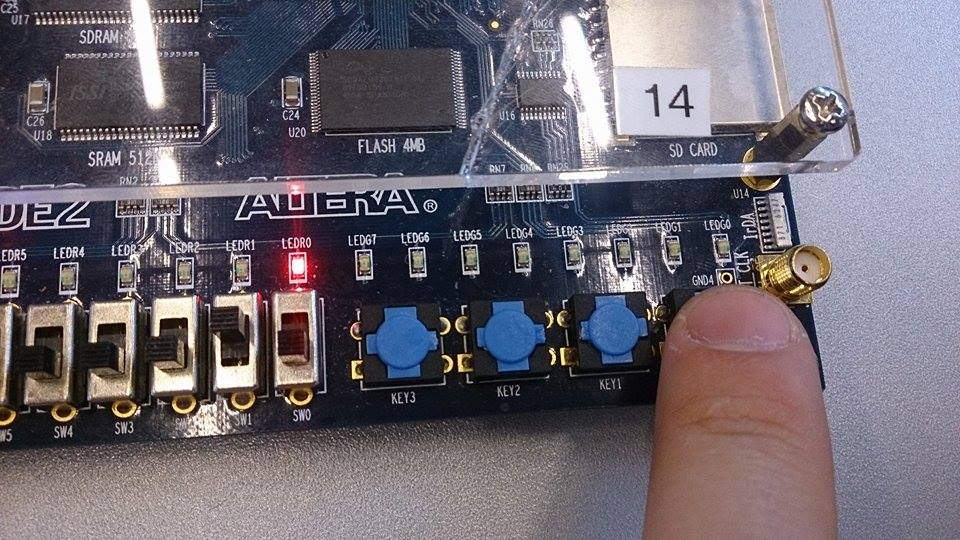
\includegraphics[scale=0.45]{pictures/Oevelse7/opg1/BA100MooMeeINIT.JPG}
	\caption{MeeMoo er i init-state og BA er 10/0}
	\label{fig:BA100MooMeeINIT}
\end{figure}
		
\begin{figure}[h]
	\centering
	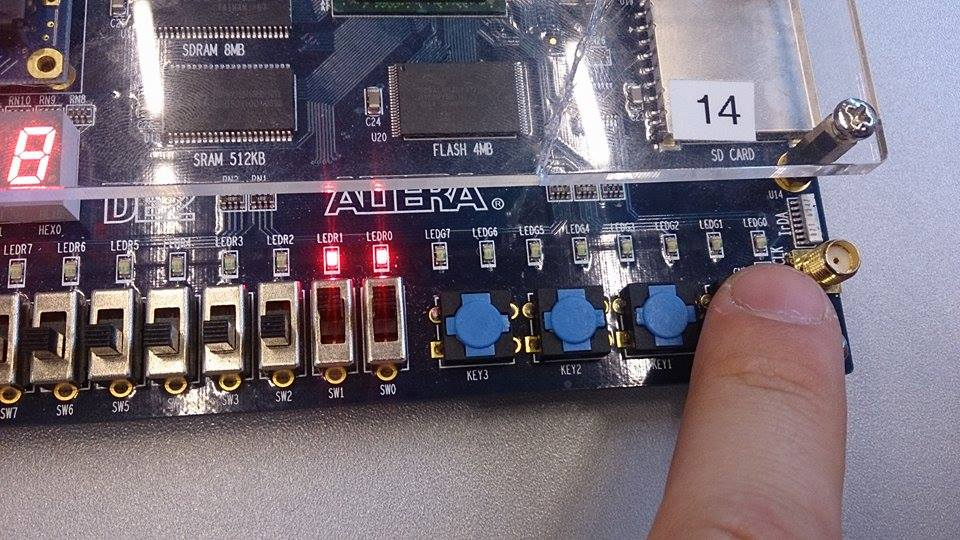
\includegraphics[scale=0.45]{pictures/Oevelse7/opg1/BA111MooMeeINIT.JPG}
	\caption{MeeMoo er i init-state og BA er 11/1}
	\label{fig:BA111MooMeeINIT}
\end{figure}


\begin{figure}[h]
	\centering
	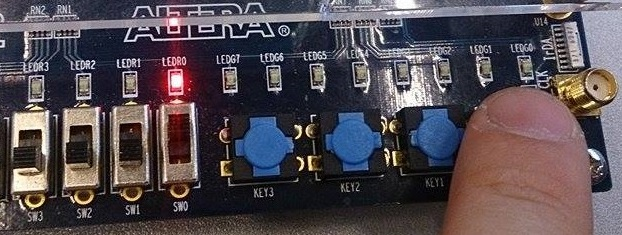
\includegraphics[scale=0.45]{pictures/Oevelse7/opg1/BA010MooMeeACTIVE.JPG}
	\caption{MeeMoo er i active-state og BA er 01/0}
	\label{fig:BA010MooMeeACTIVE}
\end{figure}

\end{enumerate}
	\newpage